\chapter{Theory}
\label{chapter:theory}

Theory is described in \gls{detail}.
For a complete understanding of the \acrshort{SRT}, one is referred to~\cite{ADP:Einstein:On_The_Electrodynamics_Of_Moving_Bodies}.

%----------------------------------------------------------------------------------------

\section{Theory: section1}
\label{section:section1}

This section stands for the theory clarification.

\subsection{Theory: subsection1}
\label{subsection:subsection1}

This subsection stands for the theory section clarification.
The formula describing the variable \(X_{Y}\) is given by the equation:

\begin{equation}
    X_Y = X + Y \text{ ,}
    \label{equation:XY_equation}
\end{equation}
where \(X\) is the variable and \(Y\) is the variable too.

\begin{align}
    X_Y =
    \tikz[baseline]{
        \node[draw=red,rounded corners,anchor=base] (m1)
        {\(\displaystyle X\)};
        \node[below of=m1] (l1) {Variable X};
        \draw[-,red] (l1) -- (m1);
    }
    +
    \tikz[baseline]{
        \node[draw=red,rounded corners,anchor=base] (m2)
        {\(\displaystyle Y\)};
        \node[below of=m2] (l2) {Variable Y};
        \draw[-,red] (l2) -- (m2);
    }
    + \ldots
    \label{equation:XY_sum}
\end{align}

Moving on to figures.
\Cref{figure:atom} illustrates the well-know \concept{atomic structure} with an \gls{atomic-mass} \glssymbol{M}.

\begin{figure}[!htb]
    \centering
    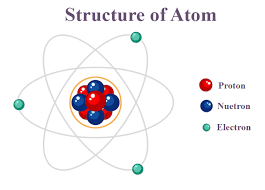
\includegraphics[width=0.9\linewidth]{Figures/Theory/atom.png}
    \caption{Atomic structure.}
    \label{figure:atom}
\end{figure}

Next two graphs show the examples of molecules.

\begin{figure}[!hbt]
    \centering
    \begin{subfigure}[b]{0.495\textwidth}
        \centering
        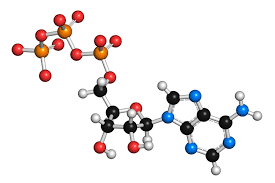
\includegraphics[width=\textwidth]{Figures/Theory/molecules.png}
        \caption{Molecules 1.}
        \label{fig:molecules1}
    \end{subfigure}
    \hfill
    \begin{subfigure}[b]{0.485\textwidth}
        \centering
        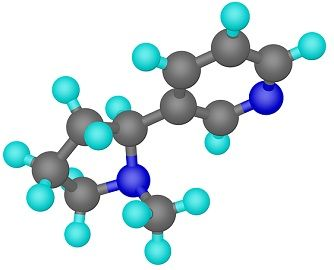
\includegraphics[width=\textwidth]{Figures/Theory/molecules1.jpg}
        \caption{Molecules 2.}
        \label{fig:molecules2}
    \end{subfigure}
    \caption{Molecules.}
    \label{fig:molecules}
\end{figure}

\subsection{Theory: subsection2}
\label{subsection:subsection2}

\begin{noteblock}
    Keeping forward.
\end{noteblock}

There were several atomic structure concepts.

Some concepts are presented in \cref{table:concepts}.
\begin{table}[!hbt]
    \centering
    \begin{tblr}{colspec={ccc}}
        \hline
        \SetCell[r=2,c=1]{m,c} Model & \SetCell[c=2]{c} Author       \\
        \cline{2,3}
                    &  Author      \\
        \hline
        Model1      &   G. Thomson    \\
        Model2      &  E. Rezerford  \\
        Model3      &   N. Bohr  \\
        Model4      &   Quantum mechanics society  \\
        \hline
    \end{tblr}
    \caption{Atomic structure models.}
    \label{table:concepts}
\end{table}

\glsresetall                                     % reset glossary entries counts for the next chapter
